\chapter{多方参与业务下的隐私保护协同计算机制}
在上一章中,我们基于隐私保护需求的多方参与业务场景构建了通用的协同计算模型,然而对于不同模块的具体交互和算法设计仍需要进一步细化。对此本章中,我们将详细讨论其内部的算法和交互策略,给出协同计算机制以支撑模型的正常运行。我们首先从交互和设计层面对协同计算模型进行划分,随后分别介绍各个模块的设计思路。

\section{基于协同计算模型的实际架构概览}
本节中,我们将对整章内容作概括性介绍,\autoref{fig:ch4-structure}给出了基于第三章中抽象模型在实际场景下的基本架构。接下来,我们将从角色分类和组成结构两部分对本架构进行介绍。
\begin{figure}[htbp]
    \centering
    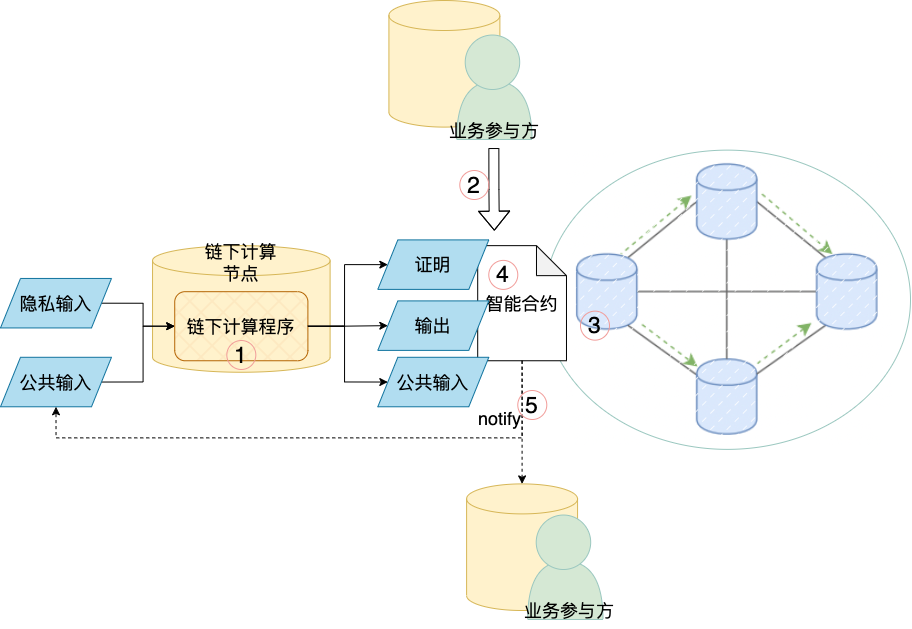
\includegraphics[width=.8\linewidth]{ch4/ch4-1}
    \caption{\label{fig:ch4-structure}基于抽象模型的协同计算架构}
\end{figure}
\subsection{角色分类}
如\autoref{fig:ch4-structure}所示,在整体架构中主要角色包括两种:业务参与方与区块链节点。其中业务参与方实际是通过链下计算节点访问在区块链节点上部署的智能合约,因此为了简化说明,我们在下文中将协同计算架构中的两种角色分别命名为链上节点和链下节点。其中链上节点间相互连接,从而共同维护整个分布式账本。与链上节点不同,链下节点之间相互独立,但其可以与某些链上节点构建连接从而向其发送交易或接收链下计算请求。

需要注意的是,虽然我们在\autoref{fig:ch4-structure}对应的协同计算架构中没有特别指明,但实际上还存在一个业务开发方的角色,其主要负责对于业务合约的设计与链下节点计算程序的设计。在后续的系统实现中为提高整个模型的通用性,我们会为其预留对应的操作接口。然而由于其并不会影响整个业务流程的运作,因此我们在本章中略去了对于这个角色的讨论。

\subsection{组成结构}
如\autoref{fig:ch4-structure}所示,我们将\autoref{fig:ch3-structure}对应的各段交互以同样的序号一一对应标注在实际的架构中,基于这一示意图,我们可以清晰地把整个机制设计划分为五个部分,其对应关系如\autoref{tab:ch4-1}所示。
\begin{table}[htbp]
    \caption{\label{tab:ch4-1}协同计算架构模块组成}
    \begin{tabularx}{\linewidth}{c|c|X<{\centering}}
        \toprule [1pt]
        \textbf{模块序号} & \textbf{抽象模型对应定义} & \textbf{实际架构对应内容} \\ \hline
        1 & \makecell[c]{业务参与方调用\\NIZK模块生成证明} & 链下节点的内部计算模块,包含隐私输入的获取、计算程序的构建与NIZK算法思路 \\ \hline
        2 & \makecell[c]{业务参与方调用\\账本模块提交交易} & 链下节点向链上节点发送交易 \\ \hline
        3 & \makecell[c]{合约状态机执行账本交易} & 链上节点的交易执行模块 \\ \hline
        4 & \makecell[c]{合约状态机调用\\NIZK模块验证证明} & 链上节点智能合约中对于NIZK验证部分的设计与调用 \\ \hline
        5 & \makecell[c]{合约状态机通知\\其他参与方执行业务} & 链上节点对链下节点的通知机制与链下节点的请求处理模块 \\
        \bottomrule [1pt]
    \end{tabularx}
\end{table}

对于模块一,即链下节点的内部计算模块,主要负责了链下的具体计算过程。简单来说,一次计算包含输入和计算程序。输入部分需要提供隐私输入和公共输入,其中公共输入为链上的账本状态,而隐私输入的获取成为了协同计算架构中需要考虑的重点。此外如2.3.3所介绍的,计算程序除了正常的执行外,还需要进行编译生成可用于NIZK算法的特定形式。与抽象模型定义相同,链下节点的计算还需要提供基于NIZK算法的证明模块。

对于模块二,即交易构建与发送等相关内容。应该包含的功能有:提供对于链上节点的API调用;对于链上合约的编译能力;对链上合约的部署和调用能力;支持构建与链上节点的通信连接等。实际上这些功能都被包含在对应的区块链系统解决方案中。以Fabric为例,其提供了Java、Go等多种语言实现的SDK实现前述特性。

同样的情况也存在于模块三,即链上节点需要提供交易的执行能力。对于不同的区块链系统交易的执行逻辑各不相同。以Fabric为例,链上节点在收到区块之后会调用区块验证器将交易从区块中逐一取出执行。根据合约的状态,执行引擎将合约执行任务分配给相应的虚拟机执行,如EVM。交易可能因Gas不足或逻辑错误等执行失败,其结果也会被封存在交易回执中。

模块四主要聚焦于链上合约的设计,对于链上合约我们需要提供针对链下计算的验证模块。除了链上节点中的NIZK算法验证模块之外,如何将验证逻辑与业务逻辑协调在一起也是设计需要考虑的问题。

对于模块五则可以细分为两个子问题,即1)基于链下计算请求的节点间交互机制;2)链下节点收到链下计算请求后的任务分配。对于子问题一,其交互包括确定链下计算请求的内容以及具体的发送流程。对于子问题二,链下节点的计算执行一般采用并发的方式,在任务分配时应注意是否存在冲突的链下计算任务。

综上,由于模块二和三主要逻辑基于特定的区块链系统提供的实现方案,因此在协同计算机制设计中我们将不过多赘述。对于模块一、四和五,在后续小节中我们将作详细介绍。

\section{链下计算}
链下节点的计算模块内部执行流程如\autoref{fig:ch4-offchain}所示,可以看到对于NIZK算法模块,其需要两部分输入:R1CS描述文件和执行计算程序后生成的witness信息。其中R1CS描述文件由编译算法生成,而witness的计算除了使用计算程序之外还包含对隐私数据的获取。接下来,本节将对各子模块作详细介绍。
\begin{figure}[htbp]
    \centering
    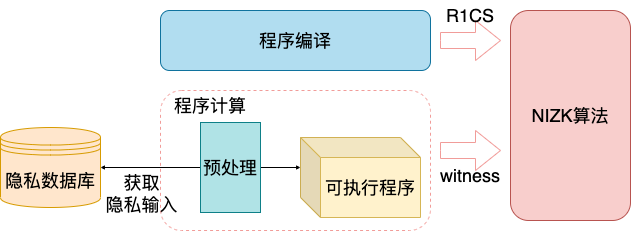
\includegraphics[width=.8\linewidth]{ch4/ch4-2}
    \caption{\label{fig:ch4-offchain}链下计算流程}
\end{figure}
\subsection{隐私数据管理}
在一般的设计中,一笔链下计算交易的创建开始于用户手动提供隐私数据输入和公开输入。然而这一设计在本文所指出的多方参与任务场景下并不适用。如第三章的抽象模型所要求的,链下节点基于链上节点发送的链下计算请求执行对应的链下计算任务,而为了保证数据隐私,链下计算请求中不应包含任何链下计算需要的隐私数据。我们可以对此作一些调整:在链下计算请求中使用隐私数据的标识符来指定其需要的隐私输入,而真正的数据存储则由链下数据源即隐私数据库负责。这样可以在保证对于链下计算请求的完整性的同时防止隐私数据的泄露。

\paragraph{设计目标} 通过对链下节点隐私数据的整体管理,我们希望实现以下几个目标:
\begin{enumerate}
    \setlength{\itemsep}{0pt}
    \setlength{\parsep}{0pt}
    \setlength{\parskip}{0pt}
    \item 隐私保护:针对多方参与业务的链下计算请求,将隐私数据的获取纳入管理可以减少数据泄露的风险;
    \item 通用性:计算任务指定需要使用的隐私数据,而链下节点维护链下数据源。如果实际的数据源发生变更,没有数据管理的缓冲将导致之前的计算任务逻辑也随之修改。使用数据管理作为中间层,有助于在连接不同链下节点和链下数据源时确保业务计算逻辑的通用性;
    \item 计算任务的稳健性:数据格式的转换是计算的前置步骤,如果交由用户完成其正确性无法保证,极有可能导致计算的错误。我们希望使用统一的数据管理确保隐私数据转换的规范性和正确性。
\end{enumerate}

\begin{figure}[htbp]
    \centering
    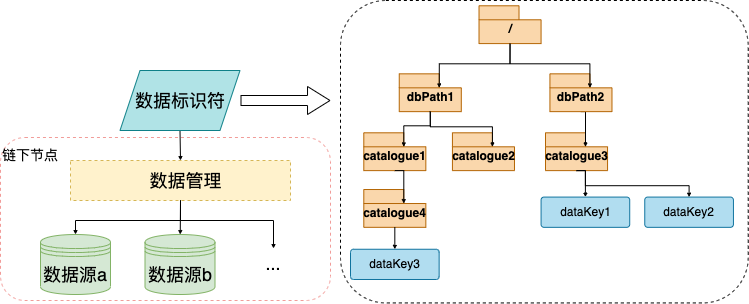
\includegraphics[width=.8\linewidth]{ch4/ch4-3}
    \caption{\label{fig:ch4-data}隐私数据管理示意图}
\end{figure}

\paragraph{数据标识符} 数据标识符是隐私数据管理中的重要概念,其连接着业务计算与具体数据源的数据项。我们将数据标识符的结构设计为:
\begin{center}
    $dbPath/catalogue_1/catalogue_2/\dots/catalogue_n/dataKey$
\end{center}
标识符的第一项$dbPath$是链下节点绑定的数据源名称,最后一项$dataKey$为数据项对应的名称,中间部分则为可以随意创建的目录项。

如\autoref{fig:ch4-data}所示,从上层的业务流程看来,整个数据管理可以看作一个虚拟文件系统。虚拟是因为其只在标识符上作声明,并不会产生真正的文件夹和数据文件。借助这一概念,我们将链下节点对数据源的管理和业务逻辑划分开来。

\paragraph{数据获取流程} 在数据管理层中,我们主要通过映射表的方式实现将标识符提供的数据标识符转换为具体的数据源存储路径。当收到链下计算请求,数据管理层将根据请求中的数据标识符和节点绑定的映射表完成对隐私数据读取路径的转换,最后根据数据源类型调用不同的底层读取模块得到隐私数据。

进一步地,我们给出链下节点在链下计算过程中的隐私数据获取流程。对于给定的隐私数据标识符及需要的计算数据格式,我们按如下步骤进行处理:
\begin{breakablealgorithm}
    \caption{隐私数据获取流程}
    \label{alg:ch4-1}
    \begin{algorithmic} 
    \item [输入]: 数据标识符$a$,目标格式$t_d$
    \STATE 根据$a_{dbPath}$在根映射表中找到对应的数据源读取实例$e$和目录映射表$table$
    \STATE 根据$table$将数据标识符$a$转换为数据源操作路径$p$
    \STATE 使用$e$读取路径$p$对应的原始隐私数据$d$和原始数据类型$t_o$
    \IF {$t_o = t_d$}
    \STATE return $d$
    \ENDIF
    \STATE 执行格式转换:$d \leftarrow transfer(d_o, t_o, t_d)$
    \STATE return $d$
    \end{algorithmic}
\end{breakablealgorithm}

\subsection{计算程序编译} 
如2.3.3所述,NIZK算法从理论上可以用于对任意NP问题论述的证明。然而对于确切的NIZK算法,其证明的论述必须基于特定的NP表示方式从而支撑算法的实际实现并保证NIZK算法的运算效率。本小节我们主要介绍在协同计算机制中对于这一预处理步骤的设计思路,我们将之称为计算程序的编译。我们首先介绍两种NP问题表示方式的基本概念和转换原理,随后给出从计算程序得到R1CS约束文件的执行流程。

\paragraph{算术电路} 我们可以把电路看作是一个有向无环图,图中节点我们称为电路的门,边则称为连接门的信号。输入信号的值经过门的计算传递到输出信号上。那么算术电路即为一类特殊的电路:所有的门的计算都是算术操作且信号的值不再只是二进制。如\autoref{fig:ch4-circuit}所示,我们给出了一个算术电路$C$的例子来说明,其中电路的输入为$\vec{i} = i_0, i_1, i_2$且输出为$\vec{o} = o_0, o_1$,而电路的中间的信号值为$\vec{w} = w_0, w_1, w_2$。

\begin{figure}[htbp]
    \centering
    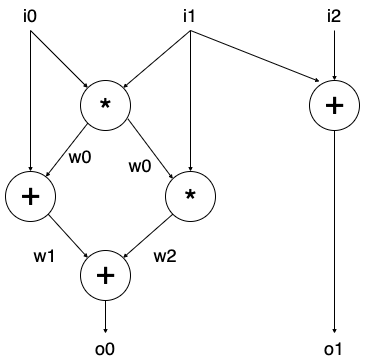
\includegraphics[width=.4\linewidth]{ch4/ch4-4}
    \caption{\label{fig:ch4-circuit}算术电路$C$示意图}
\end{figure}

对此,我们可以将\autoref{fig:ch4-circuit}中的算术电路$C$用下式表述:
\begin{equation}
    \begin{split}
    &w_0 = i_0 * i_1 \quad w_1 = i_0 + w_0 \\
    &w_2 = w_0 * i_1 \quad o_0 = w_1 + w_2 \\
    &o_1 = i_1 + i_2
    \end{split}
\end{equation}
那么我们可以得到对于算术电路的NP问题描述:当给定一部分输入信号与全部输出信号时,对于该电路是否存在一个对应的信号序列$(\vec{i}, \vec{o}, \vec{w})$?显然并没有一个有效的算法可以解决这个问题,但是当我们给出一组解$(\vec{i}, \vec{o}, \vec{w})$时,这一命题可以很快被验证是否正确。其中对应的$\vec{w}$即为该命题的witness。

\paragraph{一阶约束系统(R1CS)} R1CS是对算术电路表示的进一步优化,基于此算术电路中加法门的数量不再影响NIZK算法的计算复杂度。我们首先从简单的例子介绍。对于算术电路中的每个公式都可以使用一阶约束的形式表示,例如:
\begin{equation}
    \begin{split}
    &w_2 = w_0 * i_1 \\
    \Longleftrightarrow \quad &(1 * w_0) * (1 * i_1) = 1 * w_2 \\
    \Longleftrightarrow \quad &(
    \left( \begin{array}{ccc}
        0 \\ 0 \\ 0 \\ 0 \\ 1 \\ 0 \\ 0 \\ 0 \\ 0
        \end{array} \right), 
    \left( \begin{array}{ccc}
        1 \\ i_0 \\ i_1 \\ i_2 \\ w_0 \\ w_1 \\ w_2 \\ o_0 \\ o_1
        \end{array} \right) ) * (
    \left( \begin{array}{ccc}
        0 \\ 0 \\ 1 \\ 0 \\ 0 \\ 0 \\ 0 \\ 0 \\ 0
        \end{array} \right), 
    \left( \begin{array}{ccc}
        1 \\ i_0 \\ i_1 \\ i_2 \\ w_0 \\ w_1 \\ w_2 \\ o_0 \\ o_1
        \end{array} \right) ) = (
    \left( \begin{array}{ccc}
        0 \\ 0 \\ 0 \\ 0 \\ 0 \\ 0 \\ 1 \\ 0 \\ 0
        \end{array} \right), 
    \left( \begin{array}{ccc}
        1 \\ i_0 \\ i_1 \\ i_2 \\ w_0 \\ w_1 \\ w_2 \\ o_0 \\ o_1
        \end{array} \right))
    \end{split}
\end{equation}
而对于加法公式,我们可以通过合并同类项来消去,例如:
\begin{equation}
    \begin{split}
    & w_2 = w_0 * i_1 \quad o_1 = i_1 + i_2 \\
    \Longleftrightarrow \quad & w_0 * (o_1 - i_2) = w_2 \\
    \Longleftrightarrow \quad & 
    (0, 0, 1, 0, 0) 
    \left( \begin{array}{ccc}
        1 \\ i_2 \\ w_0 \\ w_2 \\ o_1
        \end{array} \right) *
    (0, -1, 0, 0, 1) 
    \left( \begin{array}{ccc}
        1 \\ i_2 \\ w_0 \\ w_2 \\ o_1
        \end{array} \right) =
    (0, 0, 0, 1, 0) 
    \left( \begin{array}{ccc}
        1 \\ i_2 \\ w_0 \\ w_2 \\ o_1
        \end{array} \right) \\
    \end{split}
\end{equation}

基于上述分析,我们可以给出R1CS的表示形式:
\begin{equation}
\label{equ:r1cs}
\mathbf{A}(1, \vec{i}, \vec{w}, \vec{o})^\top \odot \mathbf{B}(1, \vec{i}, \vec{w}, \vec{o})^\top = \mathbf{C}(1, \vec{i}, \vec{w}, \vec{o})^\top
\end{equation}
其中$\mathbf{A}, \mathbf{B}, \mathbf{C}$为系数矩阵,而1用于表示公式中的常量部分。对于例子$C$,其对应的R1CS表示如下。可以看到相较于算术电路表示的约束数量5,使用R1CS后NIZK算法需要证明的约束数量可以优化为2。
\begin{equation}
    \begin{split}
        \left( \begin{array}{ccccccccc}
            1 & 0 & 1 & 0 & 0 & 0 & 0 & 0 & 0 \\
            0 & 0 & 0 & -1 & 0 & 0 & 0 & 0 & 1
            \end{array} \right) (1, \vec{i}, \vec{w}, \vec{o})^\top 
        \\ \odot
        \left( \begin{array}{ccccccccc}
            0 & 1 & 0 & 0 & 0 & 0 & 0 & 0 & 0 \\
            0 & 0 & 0 & 0 & 1 & 0 & 0 & 0 & 0
            \end{array} \right) (1, \vec{i}, \vec{w}, \vec{o})^\top 
        \\ = 
        \left( \begin{array}{ccccccccc}
            0 & 0 & 0 & 0 & 0 & 0 & -1 & 1 & 0 \\
            0 & 0 & 0 & 0 & 0 & 0 & 1 & 0 & 0
            \end{array} \right) (1, \vec{i}, \vec{w}, \vec{o})^\top
        \\ (1, \vec{i}, \vec{w}, \vec{o})^\top \leftarrow 
        \left( \begin{array}{ccccccccc}
            1 & i_0 & i_1 & i_2 & w_0 & w_1 & w_2 & o_0 & o_1
        \end{array} \right)^\top
\end{split}
\end{equation}

\paragraph{编译流程} 经过上述分析,我们可以知道在链下计算过程中首先需要将链下计算程序转换为R1CS描述。在2.3.3中,我们已经对现有的NIZK编译实现作了总结。使用低级电路语言来表示计算程序可以在计算代码中对电路约束作显式声明从而让程序开发者更加明确哪些计算步骤包含在最后由R1CS描述的NP问题中,减少了由于程序编写造成的证明漏洞。此外低级电路语言更加贴近实际的电路表示形式,这有助于提高编译部分的执行效率。对此,我们基于低级电路语言来介绍整个编译流程。
\begin{enumerate}
    \item 语法生成树构建
    
    这一步骤主要目标为将读入的代码字节流转换为结构化的语法分析树用于后续的步骤处理。如\autoref{fig:ch4-ast},其内部包含两大部分:词法分析与语法分析。词法分析将源程序字符串根据构词规则分割为单词集合(Token)。语法分析则是将离散的单词集合划分为代码中的语句集合。目前已有特定的词法和语法分析自动化工具,如Lex和Yacc,因此我们在创建语法生成树时主要需要做的是在自动化工具的基础上实现对低级电路语言的关键词声明和文法构建。
    \begin{figure}[htbp]
        \centering
        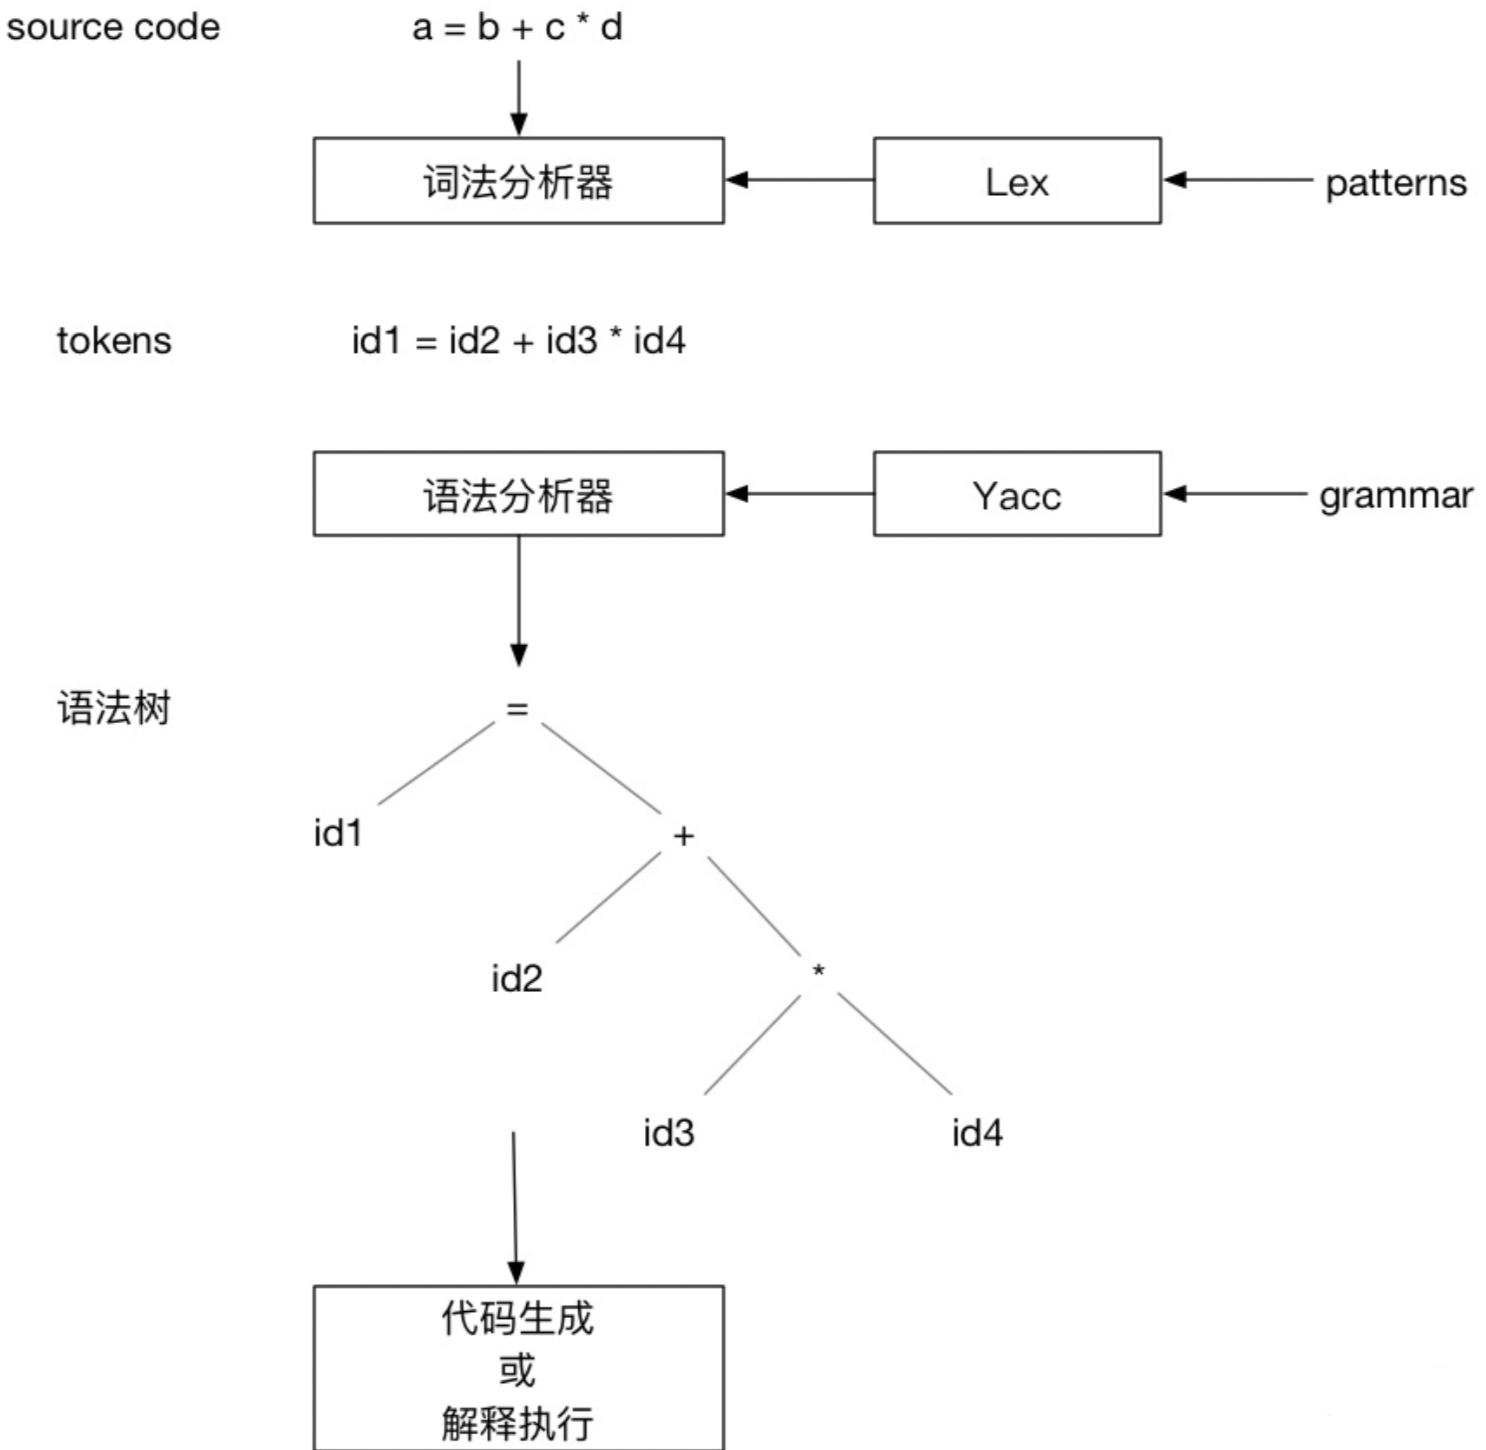
\includegraphics[width=.6\linewidth]{ch4/ch4-5}
        \caption{\label{fig:ch4-ast}语法分析树构建流程\cite{ast}}
    \end{figure}

    如\autoref{fig:ch4-ast}所示,在使用Lex构建词法分析时,我们需要自定义的部分为词法模版Patterns。Patterns规定了词法解析的具体规则,在对于低级电路语言的处理中,我们主要遵循以下规则:1)对于固定字符组成的语法关键词可以通过直接声明的方式实现;2)对于数字或是变量名等则需要通过规则匹配的形式词法分析程序将其定义为一个Token;3)对于一些特殊Token不能直接用字符串作存储,可以在识别到此类Token时追加额外的处理,例如对于数字可以将其作类型转换。

    同样地,在使用Yacc实现语法分析时,我们需要给定电路语言的具体文法Grammar。文法规则决定哪些Token组成的部分可以被规约,其工作原理为语法分析器每读取一个Token入栈检查栈中是否存在匹配的规则,存在则把匹配的部分出栈并将规约后的标识符入栈,不存在则继续移进Token。当存在规约-移进冲突时,我们可以通过定义操作符的优先级和结合性来解决冲突。在实际执行过程中,一旦分析器匹配到一条文法规则,其将执行对应的处理方法,处理的主要目标为构建一棵语法分析子树,即将匹配的Token作为子节点挂到匹配的标识符节点上。针对不同的语言,需要设计不同的语法分析树节点。\autoref{tab:ch4-2}中,我们给出了电路语言的节点结构。
\begin{table}[htbp]
    \caption{\label{tab:ch4-2}低级电路语言语法分析树节点结构表}
    \begin{tabularx}{\linewidth}{c|X<{\centering}}
        \toprule [1pt]
        \textbf{类型} & \textbf{变量名称与含义} \\ \hline
        字符串类型 & \makecell[c]{Class: 节点类型 \\ File: 引用节点用于存储对应的引用文件名 \\ OP: 操作符节点存储操作符名称 \\ DeclareType: 声明节点存储声明名称 \\ IDName: 变量节点用于存储变量名} \\ \hline
        字符串数组 & \makecell[c]{ParamNames: 函数调用节点的参数名字} \\ \hline
        节点指针 & \makecell[c]{Name: 声明节点指向其声明对象\\Block: 声明节点指向内部模块子树\\ Condition: 指向条件判断子树\\ Then: if节点的then子树\\ ElseDo: if节点的else子树\\ Init: 循环节点的初始化子树\\ Step: 循环节点的循环处理子树\\ Body: 当前节点的内部语句块子树\\ Value: 返回节点对应的表达式子树\\Component: 当前节点的函数调用子树\\ Pin:当前节点的变量访问子树} \\ \hline
        布尔类型 & \makecell[c]{Private: 变量节点是否为隐私输入} \\ \hline
        节点指针数组 & \makecell[c]{Params: 函数调用节点的参数节点\\Values: 操作符或数组变量对应的具体数值 \\ Expressions: 当前节点的表达式子树\\Statements:Block节点下的语句子树} \\ \hline
        数值类型 & \makecell[c]{RefID: 实例分析中使用的id\\NumValue:具体数值} \\ \hline
        数值数组 & \makecell[c]{SymbolRange: 指明当前节点在字节流中的位置} \\
        \bottomrule [1pt]
    \end{tabularx}
\end{table}
    \item 实例分析
    
    通过深度优先遍历生成的语法树,我们可以分析出代码中实际存在声明创建的实例。在实例分析中我们主要完成以下步骤:1)识别代码中创建的所有实例,包含对函数实例和变量、信号实例;2)根据上下文分析实例的作用域,并对同一作用域内的实例进行编号和实例对象创建,其编号被记录在\autoref{tab:ch4-2}的RefID中;3)对于引用文件,读入其对应代码字节流并进行语法分析树的构建和统一的实例分析。
    
    对于步骤1,我们可以在后续的分析中,将计算的执行和约束的构建转换为对具体实例的操作处理上,也可以完成对电路中信号的初步识别。而步骤二可以在后续的分析中很快检查出代码语义是否出错,即是否在实例作用域外出现对该实例的引用。步骤3主要是对于外部引用的处理,在这一步中我们可以将多个文件构建的代码合并在一个语法分析树和实例系统中。
    \item 约束构建
    
    整个约束构建实际上在对语法分析树进行深度优先的后序遍历算法基础上在遍历到每个节点时增加了对实例的处理。从执行的角度上,我们可以把代码中的所有语句简单划分为两类:计算赋值语句和其他语句。
    
    其他语句包含声明、调用和语法糖,虽然它们本身没有具体的计算赋值,但是这类节点一定包含内部语句块,使用节点指针或节点指针数组类型的变量指向一组计算赋值语句。对于其他语句的处理一般会直接继续深度遍历其子树,但是需要特别注意的是条件判断和循环语句这两种。条件判断和循环语句如果包含电路约束,我们要求其执行路径必须在编译时确定。这一要求是与电路约束所代表的NP问题相关联的,如果在编译时无法确定执行路径这意味着我们无法将该代码拍平成一个确定的算术电路,那么显然约束也无从谈起。因此对于无法确认的条件转移,我们在遍历时会直接跳过,这也是我们推荐使用低级电路语言编写计算程序的原因。程序开发者如果在这类语句中声明了一个电路约束,在编译过程中由于无法确定算术电路我们将返回报错。

    对于计算赋值语句,我们的核心思路就是将计算结果附加在被赋值的实例对象中。如果计算结果可以在编译时确定,我们在实例中记录具体数值,而如果需要执行时确定,我们直接将表达式记录下来。所有声明约束的语句都是计算赋值语句,因此当识别到其为约束时,我们将语句中的实例及其表达式合并为一个一阶约束,并记录到约束表中。
    \item 主模块检查
    
    主模块检查的主要功能就是确认整个计算程序的入口,以类C的低级电路语言为例,主模块即为main函数。这一检查的实现思路也较为简单,在实例分析中,我们已经对所有的函数和变量作记录,因此在检查时只需要遍历整个实例对象表即可确认是否有对应的主模块。
    \item 信号分析
    
    信号分析作为整个编译算法的收尾部分主要将电路中的所有信号进行整理。在实例分析中,我们把所有的变量都看作是实例对象,而实际上并不是所有的变量都会包含在最后的R1CS中,其中很多都是方便计算的中间变量。此外变量和信号在语义中并不等价,根据算术电路的特性,我们可以发现信号的值不会改变,是一类特殊的变量。在低级电路语言中,我们可以对此作显式的区分,从而让信号分析更为高效。而变量主要用于一些复杂的运算操作,由于算术电路和R1CS都只支持了乘法和加法,因此例如指数、取模等运算我们可以借用变量作计算,当然需要注意无法在编译时确定的这类计算也将无法被电路约束。

    信号分析的核心思路为将现有的信号实例与约束分析中得到的约束信息作对照:1)只有那些出现在约束中的信号被统计在最后的信号表中;2)优化信号间的赋值导致的多个信号。步骤2中的优化思路可以描述为:根据信号的实例表达式,我们可以发现相互赋值的操作,从而识别到共存的同一信号值;在消去时我们优先保留外部输入信号和输出信号,从而减少内部信号的存在;在消去时,我们也相应地更新约束信息,使得约束信息与信号表保持一致。
\end{enumerate}

\subsection{基于Groth16的NIZK算法模块}
在2.1.6中我们对链下计算使用的技术方案进行了详细的分析比较,并且认为zk-SNARKs是一种较为理想的解决方案。因此在协同计算机制中,我们采用了zk-SNARKs中的Groth16算法\cite{cryptoeprint:2016/260}。该算法生成的证明大小和验证复杂度均为$O(1)$,其中证明只包含了三个参数,可以认为是目前在性能上表现最优的zk-SNARKs算法。在本小节中我们将对Groth16的算法流程作介绍。
\paragraph{R1CS与QAP问题的转换}
在Groth16中需要将如\autoref{equ:r1cs}所表示的R1CS形式转化为QAP问题。正如4.2.2算术电路中所介绍的,算术电路和R1CS描述的NP问题为给定一部分信号值,是否有对应的内部信号值满足该电路。我们可以将这一问题表示为:
\begin{equation}
    \label{equ:rInCircuit}
    R = \left \{ \begin{array}{c|l}
        (\varphi, \omega) 
        & \begin{array}{l}
            \varphi = (s_1, \dots, s_l) \in \mathbb{F}^l \\ 
            \omega = (s_{l+1}, \dots, s_m) \in \mathbb{F}^{m-l} \\
            \mathbf{A}(s_0, s_1, \dots, s_m)^\top \odot \mathbf{B}(1, s_1, \dots, s_m)^\top = \mathbf{C}(1, s_1, \dots, s_m)^\top
        \end{array}
    \end{array} \right \}
\end{equation}
其中$\mathbb{F}$为有限域,$(s_0, \dots, s_m), s_0 = 1$为电路中的全部信号,$\mathbf{A}, \mathbf{B}, \mathbf{C}$为系数矩阵,$\varphi$为statements,$\omega$为witness,$l, m$由算术电路规模决定。

Gennaro\cite{gennaro2013quadratic}指出当$\mathbb{F}$足够大时,我们可以将\autoref{equ:rInCircuit}中的第三个等式转换为QAP。当我们将系数矩阵按行拆分时,该等式可以看作以$\sum s_i a_{i,q} \cdot \sum s_i b_{i, q} = \sum s_i c_{i, q}, i \in m, q \in n$形式表示的等式组,其中$n$为约束数量,即系数矩阵的行数。进一步地,我们取$(r_1, \cdots, r_n) \in \mathbb{F}$,并构建$n-1$次多项式$u_i(x), v_i(x), w_i(x)$满足映射关系:$u_i(r_q) = a_{i, q}, v_i(r_q) = b_{i, q}, w_i(r_q) = c_{i, q}$。那么当$t(x) = \prod\limits_{q=1}^n(x-r_q)$时,一定存在$h(x)$满足\autoref{equ:qap}。
\begin{equation}
    \label{equ:qap}
    \sum\limits_{i=0}^m s_i u_i(X) \cdot \sum\limits_{i=0}^m s_i v_i(X) - \sum\limits_{i=0}^m s_i w_i(X) = h(X)t(X)
\end{equation}

综上,我们可以将Groth16所需的NP问题表示为:
\begin{equation}
    R = \left \{ \begin{array}{c|l}
        (\varphi, \omega) 
        & \begin{array}{l}
            \varphi = (s_1, \dots, s_l) \in \mathbb{F}^l \\ 
            \omega = (s_{l+1}, \dots, s_m) \in \mathbb{F}^{m-l} \\
            \sum\limits_{i=0}^m s_i u_i(X) \cdot \sum\limits_{i=0}^m s_i v_i(X) - \sum\limits_{i=0}^m s_i w_i(X) = h(X)t(X)
        \end{array}
    \end{array} \right \}
\end{equation}
\paragraph{Groth16算法流程} 整个算法流程可以分为可信设置setup阶段,证明过程prove和验证过程verify。Groth16的可信设置是针对每个电路生成的,其生成的数据将作为证明密钥$pk$和验证密钥$vk$用于后续的证明和验证中。
\begin{enumerate}
    \item setup: 从有限域$\mathbb{F}$中选取随机值$\tau = (\alpha, \beta, \gamma, \delta, x)$,并生成
    \begin{equation}
        \begin{split}
        \left \{x^i \right \}_{i=0}^{n-1}, 
        \left \{ \frac{\beta u_i(x)+\alpha v_i(x) + w_i(x)}{\gamma}\right \}_{i=0}^l, 
        \\
        \left \{ \frac{\beta u_i(x)+\alpha v_i(x) + w_i(x)}{\delta}\right \}_{i=l+1}^m,
        \left \{ \frac{x^i t(x)}{\delta}\right \}_{i=0}^{n-2}
    \end{split}
    \end{equation}
    将这些参数映射到椭圆曲线$G_1, G_2$上构建$pk, vk$
    \item prove: 证明包含$A, B, C$三个参数,在计算前证明方从有限域$\mathbb{F}$中选取随机值$r, s$,构造证明如下
    \begin{equation}
        \begin{split}
        & A = \alpha + \sum \limits_{i=0}^m a_i u_i(x) + r \delta \quad B = \beta + \sum \limits_{i=0}^m a_i v_i(x) + s \delta
        \\
        & C = \frac{\sum \limits_{i=l+1}^m a_i (\beta u_i(x)+\alpha v_i(x) + w_i(x)) + h(x)t(x)}{\delta} + As + rB - rs\delta
    \end{split}
    \end{equation}
    \item verify: 验证\autoref{equ:verify}是否成立
    \begin{equation}
        \label{equ:verify}
        A \cdot B = \alpha \cdot \beta + \frac{\sum \limits_{i=0}^l a_i (\beta u_i(x)+\alpha v_i(x) + w_i(x))}{\gamma} \cdot \gamma + C \cdot \delta
    \end{equation}
    
\end{enumerate}

\section{链上验证}
为了通用性的需求,我们将验证和业务逻辑分离开来,从而使得链上业务与对链下计算验证的变动完全独立开来,这样一方的修改不会对其他业务部分造成过多影响。如\autoref{fig:ch4-verify}所示,我们将链上合约设计为业务部分和验证部分,其中请求的打包和处理看一看作是对同一链下计算任务实例的对等解析过程,从而将业务的回调相关信息传递到验证逻辑中。接下来,我们首先介绍满足这一传递机制的相关数据结构,随后给出整个链上合约的验证调用流程。
\begin{figure}[htbp]
    \centering
    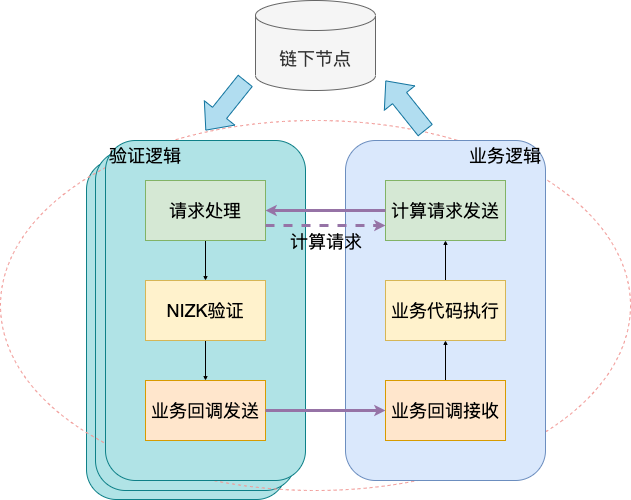
\includegraphics[width=.6\linewidth]{ch4/ch4-6}
    \caption{\label{fig:ch4-verify}链上合约示意图}
\end{figure}

\subsection{数据结构} 整个链上合约验证流程中的数据结构可以从功能角度分为两类,一类为对链下计算信息的存储,另一类用于构建业务与验证之间连接。链下计算信息包含:
\begin{itemize}
    \setlength{\itemsep}{0pt}
    \setlength{\parsep}{0pt}
    \setlength{\parskip}{0pt}
    \item 链下计算标识$circuitId$:与链下节点的链下计算程序相对应,当验证合约收到链下计算证明时首先需要验证是否为对应的cricuitId
    \item NIZK验证密钥$vk$:合约对应的链下计算程序在setup阶段得到的验证密钥
    \item 链下计算任务$tasks$:保存链下计算任务与其相关计算信息的映射关系
\end{itemize}
链下计算标识和验证密钥将在初始化时作为固定值保存在合约中,而链下计算任务的存储则是在合约执行中动态添加的。除此之外,请求结构体则是合约构建计算请求和解析验证请求的模版结构,主要内容包括:
\begin{itemize}
    \setlength{\itemsep}{0pt}
    \setlength{\parsep}{0pt}
    \setlength{\parskip}{0pt}
    \item 计算请求结构体$eventCompute$:
    \\ \textbf{单次计算标识$taskId$}:用于标识一次链下计算任务实例
	\\\textbf{链下计算标识$circuitId$}:指明请求的链下计算程序
	\\\textbf{业务回调地址$addr$}:记录业务回调地址,用于链上验证处理阶段
	\\\textbf{链下计算输入$input$}:链下计算输入包含公开输入$pub$和隐私输入$priv$,公开输入直接提供数值,而隐私输入使用4.2.1提供的标识符形式指明
    \item 验证请求结构体$eventVerify$:
    \\\textbf{单次计算标识$taskId$}:用于标识一次链下计算任务实例,对于一组计算请求和验证请求,其$taskID$应保持相等
    \\\textbf{计算结果$result$}:链下计算结果
    \\\textbf{NIZK证明$proof$}:链下计算对应NIZK证明
\end{itemize}

\subsection{链上合约验证流程}
如\autoref{fig:ch4-verify}所示,从链上验证逻辑来看,外部输入主要有两个:业务逻辑向其申请构建计算请求,链下节点发起的验证请求。因此在\autoref{alg:ch4-2}中我们分别给出其对应的内部处理流程,其中$cid$为当前合约对应的链下计算程序标识,$cvk$为当前合约对应的链下计算setup得到的验证密钥。
\begin{breakablealgorithm}
    \caption{链上合约验证流程}
    \label{alg:ch4-2}
    \begin{algorithmic} 
    \item [初始状态]: $circuitId \leftarrow cid, vk \leftarrow cvk, tasks \leftarrow \epsilon$
    \item [构建计算请求]: $w(pub, priv), addr$
    \STATE 随机选取字符串$v$,满足$tasks[v] = \perp$
    \STATE let $taskId \leftarrow v, input \leftarrow w$
    \STATE let $q \leftarrow (taskId, circuitId, addr, input)$
    \STATE $tasks[taskId] \leftarrow (addr, pub)$
    \STATE return $q$
    \item [收到验证请求]: $taskId, proof, result$
    \IF {$tasks[taskId] = \perp$}
    \STATE return $\perp$
    \ENDIF
    \STATE let $(addr, pub) \leftarrow tasks[taskId]$
    \STATE 调用NIZK$verify: vk, \varphi(pub, result), proof$,返回$b$
    \IF {$b = \perp$}
    \STATE 回调业务逻辑$invoke: addr, taskId, \perp$
    \STATE return $\perp$
    \ENDIF
    \STATE 回调业务逻辑$invoke: addr, taskId, result$
    \STATE return $\top$
    \end{algorithmic}
\end{breakablealgorithm}

\section{链下计算请求}
如前文所述,链下计算请求的处理实际上可以被分为两部分。一部分是链上节点与链下节点间关于链下计算请求的交互逻辑,在4.3中我们对于计算请求的构建流程进行了详细的介绍,4.4.1中我们将继续介绍\autoref{fig:ch4-verify}中业务逻辑在收到构建好的链下计算请求后其请求发送部分的逻辑。另一部分为链下节点对于收到链下计算请求后的处理流程,在4.2中我们已经介绍了链下计算的执行逻辑但是链下节点在任务调度上的逻辑仍需进一步讨论,我们将在4.4.2中给出相应的算法。
\subsection{链下计算请求交互机制}
基于多方参与的业务场景,我们允许业务逻辑中出现对于其他链下节点计算的调用请求,通过这一方式将其他业务参与方纳入业务流程中。在业务执行时如果遇到对链下计算请求的声明,其执行流程为:1)将声明内容传递给相应验证逻辑并得到构建完成的链下计算请求;2)推送消息到目标节点

对于步骤一,在4.3.2中我们已经介绍了验证逻辑中构建计算请求需要的输入,即$w(pub, priv), addr$。因此在业务逻辑设计中,我们要求每个对链下计算请求的声明都必须包含这些内容,即业务逻辑中的声明对应数据结构为:
\begin{itemize}
    \setlength{\itemsep}{0pt}
    \setlength{\parsep}{0pt}
    \setlength{\parskip}{0pt}
    \item 链下计算公开输入$pub$:数值形式给定的输入内容
    \item 链下计算隐私输入$priv$:4.2.1标识符形式给定的输入内容
    \item 业务回调地址$addr$:当链下计算完成后需要继续执行的下一步业务内容对应合约和函数地址
\end{itemize}

对于步骤二,推送的正常执行实际上由链下节点和链上节点共同保证。首先,为了保证请求正确送达目标链下节点,我们要求链下节点要提前注册对相应事件的监听。其次,链上节点在合约执行中将步骤一得到的链下计算请求作为内容触发合约事件。
\subsection{链下节点的任务分配}
链下节点的任务分配其目标就是在收到链下计算请求后在合适的时机调用链下计算程序完成计算。显然在简单场景下,链下节点每收到一个链下计算请求可以直接将其移交到4.2给出的链下计算逻辑中。

然而在多请求场景下,情况开始变得复杂,一个简单的例子就是:链下节点存放了a=1, b=0, c=0, 此时a给b转账1,b再给c转账1。显然此时如果调换两次计算的前后顺序,b给c的转账将直接失败。针对此,我们给出链下计算请求依赖性定义:对于链下节点$p$其对应链下合约状态为$\rho[p]$,存在两个链下计算请求$q_a, q_b$,同样以$\rho[p]$作为初始状态按照$q_a, q_b$和$q_b, q_a$的顺序分别完成计算后的链下合约状态为$\rho[p]_1, \rho[p]_2$。一旦$\rho[p]_1, \rho[p]_2$不相等,我们认为这两个链下计算请求是存在依赖的。

当然一种简单的策略即为强制所有的链下计算任务串行化执行,当收到一个链下计算请求后将其对应任务放入队列尾部,只有在一个任务计算完成后再从队列头部取出下一个计算任务。遗憾的是这一方案将极大影响整体的业务执行性能,因此我们考虑在任务分配机制中加入计算依赖性分析来支持对于链下计算的并发并行执行。

基于依赖性分析的链下节点任务分配流程如\autoref{alg:ch4-3}所示。每当收到一个链下计算请求时,我们计算其在当前未完成任务中的依赖请求,并更新相关的全局变量。当计算任务执行完毕或存在空闲的计算实例时,我们尝试找到一个未完成且未在计算中的计算任务移交给计算实例,其满足没有前置依赖的要求。对于依赖分析函数$dep$,其主要逻辑为将请求与未完成任务中所有请求作比对,检查预编译的计算程序是否涉及状态转移的冲突,从而找到所有依赖请求。
\begin{breakablealgorithm}
    \caption{链下节点任务分配流程}
    \label{alg:ch4-3}
    \begin{algorithmic} 
    \item [初始状态]: 
    \\ $U \leftarrow \epsilon$, 存放未完成的计算任务
    \\ $workList \leftarrow \epsilon$, 存放执行中的计算任务
    \\ $TaskRef \leftarrow \epsilon$, 存放映射关系:计算任务 $\leftarrow$ 依赖的任务集合
    \\ $TaskDep \leftarrow \epsilon$,存放映射关系:计算任务 $\leftarrow$ 依赖于该任务的任务集合
    \item [收到链下计算请求]: $q(taskId, circuitId, addr, input)$
    \STATE $U \leftarrow U \parallel q$
    \STATE let $d \leftarrow dep(q)$
    \STATE $TaskRef[q] \leftarrow d$
    \FOR {$q_d \in d$}
    \STATE $TaskDep[q_d] \leftarrow TaskDep[q_d] \parallel q$
    \ENDFOR
    \STATE return
    \item [收到任务完成回调]: $q(taskId, circuitId, addr, input)$
    \STATE $U \leftarrow U / q, workList \leftarrow workList / q$
    \STATE let $d_u \leftarrow TaskRef[q]$
    \STATE $TaskDep[q] \leftarrow \perp$
    \FOR {$q_u \in d_u$}
    \STATE $TaskRef[q_u] \leftarrow TaskRef[q_u] / q$
    \ENDFOR
    \FOR {$q_t \in U$}
    \IF {$q_t \in workList$}
    \STATE continue
    \ENDIF
    \IF {$TaskRef[q_t] = \perp $}
    \STATE 将$q_t$移交给计算逻辑
    \STATE $workList \leftarrow workList \parallel q_t$
    \STATE return
    \ENDIF
    \ENDFOR

    \noindent\hrulefill
    \item [$dep(q)$]:
    \STATE let $Q \leftarrow \epsilon, (\cdot, circuitId, \cdot, input) \leftarrow q$
    \FOR {$q_u \in U$}
    \STATE let $(\cdot, circuitId_u, \cdot, input_u) \leftarrow q_u$
    \IF {$circuitId_u$对应逻辑存在对$input$的修改 $\vee$ $circuitId$对应逻辑存在对$input_u$的修改}
    \STATE $Q \leftarrow Q \parallel q_u$
    \ENDIF
    \ENDFOR
    \STATE return $Q$
    \end{algorithmic}
\end{breakablealgorithm}